\subsection{Architecture Verification}

[JUNAID/ISAAC - 1 pg]

AGREE analysis of RTA arch in AADL

One of the steps in constructing the assurance argument of the RTA architecture is verifying the architecural model with respect to formal high-level requirements.
The RTA architecture was modelled in AADL (Fig. \ref{fig:rta-agree}) using the Open Source AADL Tool Environment (OSATE),
and the high-level requirements were added to this AADL model as AGREE specifications \cite{agree2012}.
AGREE specifications are used to describe component behavior through assume-guaranteee contracts, and
these contracts are analyzed using AGREE's compositional reasoning framework available through the AGREE plugin for OSATE.
[TODO: do we need to describe AADL here?]
[TODO: do we need to mention FMIDE?]

The goal of the AGREE analysis of the RTA architecture was to verify the following high-level property:
the RTA architecture is guaranteed to publish only safe flight plans.
[TODO: Isaac, please edit the requirement wording]
In Fig. \ref{fig:rta-agree}, when an avoidance alert is generated, the Safe Backup Planner generates a BAF plan;
this triggers the generation of an LEC plan.
The Plan Selector chooses one of the two plans based on the SWC Assessment output, and informs the Plan Switch of its decision.
The Plan Switch publishes a flight plan based on the Plan Selector output.
We annotated the RTA's AADL model with assume-guarantee contracts for each of the RTA architecture components,
and the AGREE plugin was able to verify the high-level property under the assumption that BAF flight plans were safe.

\begin{figure*}
	\centering
	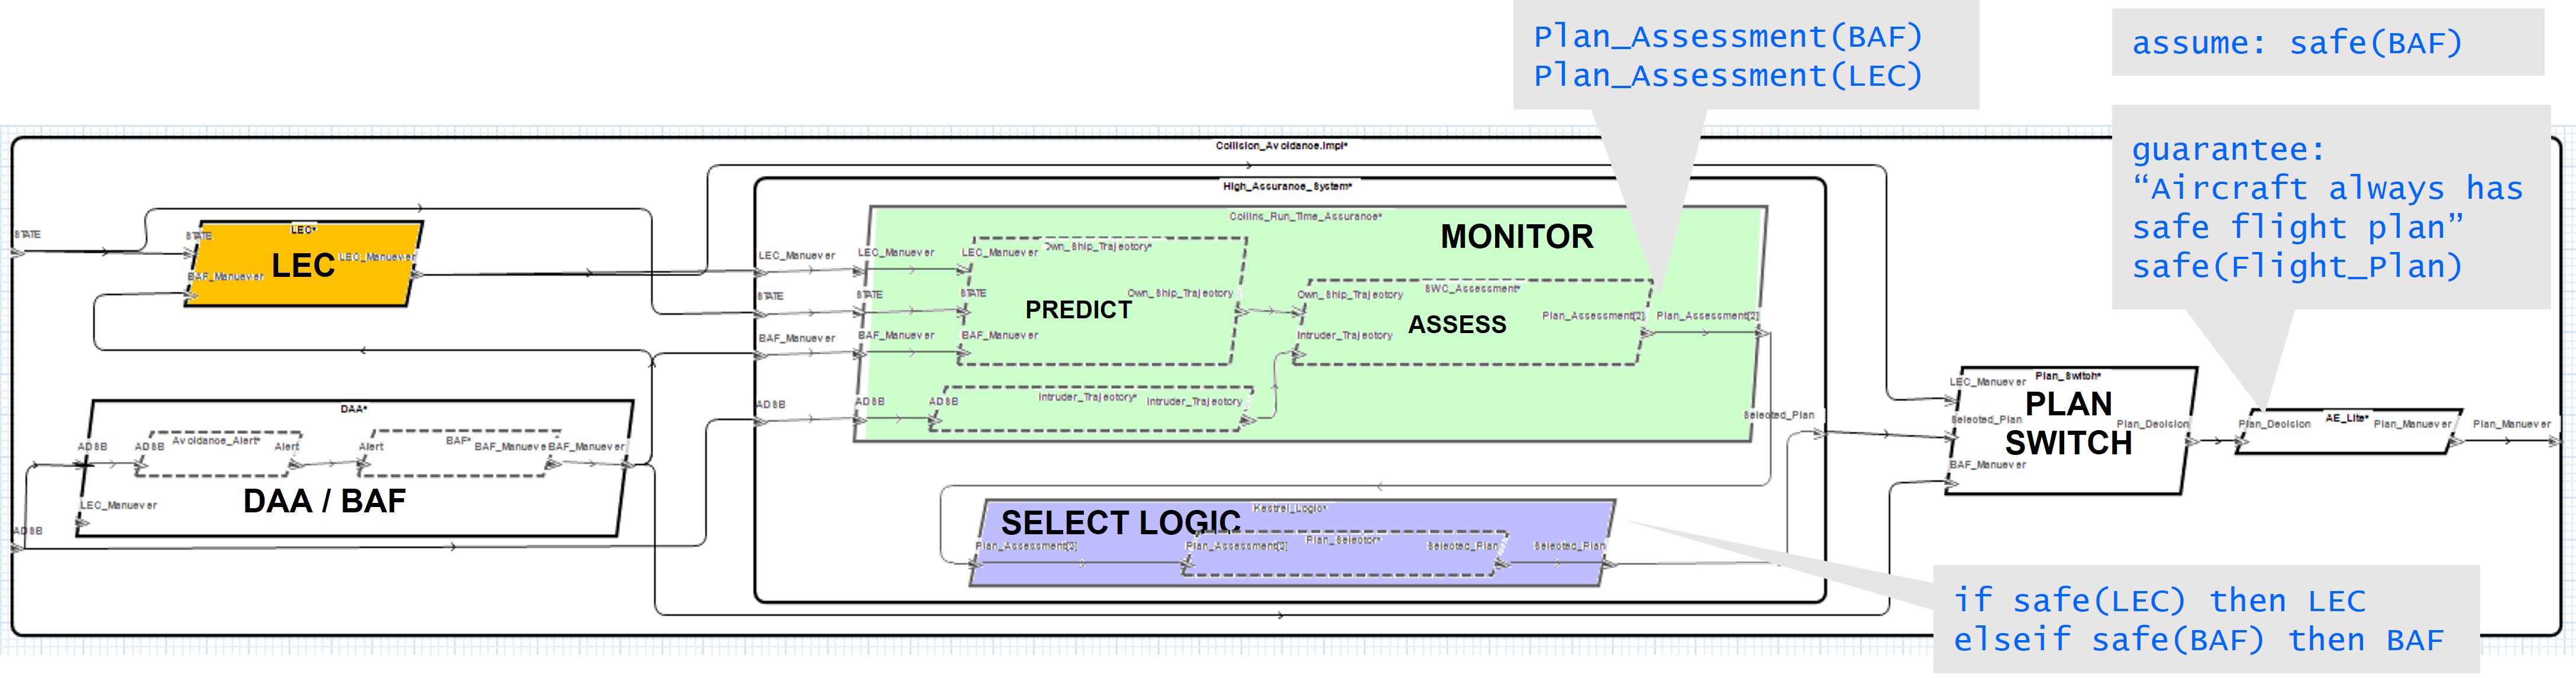
\includegraphics[width=\textwidth]{figures/rta-agree.jpg}
	\caption{AADL Model of Run-Time Assurance Architecture and AGREE properties}
	\label{fig:rta-agree}
\end{figure*}